%%%%%%%%%%%%%%%%%%%%%%%%%%%%%%%%%%%%%%%%%%%
%        Packages utilisés                %
%%%%%%%%%%%%%%%%%%%%%%%%%%%%%%%%%%%%%%%%%%%



	%[twoside,12pt]

	%\documentclass[french,12pt]{report} %pour une police de 12 au cas où
	\documentclass[french]{book} %{report}


	\usepackage[T1]{fontenc}
	\usepackage[utf8]{inputenc} %Permet d'utiliser des caractères spéciaux : éèàçù etc. plus sûr que \usepackage[latin9]{inputenc}
	%\usepackage[latin9]{inputenc}

	\usepackage[french]{babel}
	\usepackage{geometry} %Personnaliser l'aspect géométrique du document.
	\geometry{top=3cm, bottom=3cm, left=3cm , right=3cm} %plus simple que le suivant, que je ne maîtrise pas...
	%\geometry{verbose,tmargin=2.5cm,bmargin=2.5cm,lmargin=1.5cm,rmargin=1.5cm,headheight=2.5cm,headsep=2.5cm,footskip=2.5cm}
	
	\usepackage{amstext} 
	\usepackage{graphicx} 
	\usepackage{amssymb} 
	\usepackage{hyperref} %Celui-là il est surpuissant : il fait tous les liens hypertexte et intratexte. [hidelinks]==> pas de couleur 
	%\hypersetup{colorlinks=false }
	%\hypersetup{hidelinks}


	\usepackage[footnotesize]{caption} 
	\usepackage{amsmath, amssymb} 
	\usepackage{color} 
	%\usepackage{times} %permet de choisir la police, mais la Latin Modern me convient. 
	%\usepackage{fullpage} %définit tout une mise en page qui bousille le package geometry !!!! ==> je ne l'utilise pas.

	\usepackage{natbib} 
	\usepackage{colortbl}

	\usepackage[french]{minitoc} 
	\usepackage{tocloft}  
	\usepackage{titletoc}  
	\usepackage{appendix} 
	\usepackage{eurosym} % pour ajouter le symbole € en tapant \euro
	\usepackage{colortbl} 
	\usepackage{lipsum}
	\usepackage{amsthm} %théorèmes, etc.
	\usepackage{stmaryrd} %crochets d'entiers
	\usepackage{empheq} %équations encadrées
	\usepackage{mathrsfs}  %zoulies majuscules avec la commande \mathscr{}

	\usepackage{yfonts} %gothique ; utiliser la commande : \textgoth{ABCdef123} ou \textswab{ABCdef123}.

	\usepackage{bm} %\bm{truc} = truc en gras mais avec la bonne police
	%\usepackage{frbib} %Bibliographie en français

	\usepackage{epigraph}
	%\epigraphfontsize{\small\itshape}
	\setlength\epigraphwidth{8cm}
	\setlength\epigraphrule{0pt}



	\makeatletter




	%%%%%%%%%%%Commandes pour la bibliographie.
		\def\aj{\textit{The Astronomical Journal}}


		\def\nat{\textit{Nature}}
		\def\icarus{\textit{Icarus}}
		\def\aap{\textit{Astronomy and Astrophysics}}
		\def\grl{\textit{Geophysical Research Letters}}
		\def\jgr{\textit{Journal of Geophysical Research}}





	\newcommand{\figpath}{figures/}
	\newcommand{\bibpath}{/Volumes/USER/robutel/Phil/Articles/base/}






	\makeatother



	\newcommand{\HRule}{\rule{\linewidth}{0.5mm}}


	%%%%%%%%%%%%%%%%%%%%%%%%%%%%%%%%%%%%%%%%%%%%%%
	%Théorèmes, démonstrations, etc.
	%
	%%%%%%%%%%%%%%%%%%%%%%%%%%%%%%%%%%%%%%%%%%%%%

	\newtheorem{post}{Postulat}[section]
	\newtheorem{theorem}{Theorème}[section]
	\newtheorem{lemma}{Lemme}[section]
	\newtheorem{definition}{Définition}[section]
	\newtheorem{cor}{Corrolaire}[section]
	\newtheorem{prop}{Proposition}[section]
	\newtheorem{conj}{Conjecture}[section]
	\theoremstyle{plain}
	\renewcommand{\qedsymbol}{\textit{Q.E.D.}}




	%%%%%%%%%%%%%%%%%%%%%%%%%%%%%%%%%%%%%%%%%%ù
	%
	%typographie matheuse
	%
	%%%%%%%%%%%%%%%%%%%%%%%%%%%%%%%%%%%%%%%%%%

    %\newcommand{\d}{\mathop{}\mathrm{d}}
	\def\d{\mathrm{d}}
	\def\e{\mathrm{e}}
	\def\i{\mathrm{i}}


	\def \eps {\varepsilon}
	\def\percent{\%}
	\def\etal{{et al.}}





	%%%%%%%%%%%%%%%%%%%%%%%%%%%%%%%%%%%%%%%%%%%%%
	%bas de page, haut de page
	%        etc.
	%		Plüthaar.
	%%%%%%%%%%%%%%%%%%%%%%%%%%%%%%%%%%%%%%%%%%%%%

	%\renewcommand{\headrulewidth}{1pt}
	%\fancyhead[C]{\textbf{page \thepage}} 
	%\fancyhead[L]{\leftmark}
	%\fancyhead[R]{machin}

	%\renewcommand{\footrulewidth}{1pt}
	%\fancyfoot[C]{Léo BERNUS} 
	%\fancyfoot[L]{truc}
	%\fancyfoot[R]{\leftmark}



\begin{document}

%%%%%%%%%%%%%%%%%%%%%%%%%%%%%%%%%%%%%%%%%%%%%%%%%%%%%%%%%%%%%%%%%%%%%%
%                                                                    %
%                          Page de garde                             %
%                                                                    %
%%%%%%%%%%%%%%%%%%%%%%%%%%%%%%%%%%%%%%%%%%%%%%%%%%%%%%%%%%%%%%%%%%%%%%




	\begin{titlepage}

	\begin{center}


	%%%%%%%%%%%%%
	%  Logos    %
	%%%%%%%%%%%%%

	%On s'en occupera plus tard.


	\begin{center}
		%\includegraphics[width = 40mm]{../logos/SANSELIPS.jpg} \hfill
		%\includegraphics[width = 40mm]{../logos/logo_IMCCE_small.jpg} \hfill
		%\includegraphics[width = 40mm]{../logos/logo_iap.jpg} \hfill
		%\includegraphics[width = 40mm]{../logos/UPMC_pantones_7504-166.jpg} \hfill    

	\end{center}





	%%%%%%%%%%%%%%%%%%%%%%%%%%%%%%%%%%%%%%%%%%%%%%%%%%%%%%%%%%%%%%%%%
	%   Code pour zoulie page de garde.                             %
	%%%%%%%%%%%%%%%%%%%%%%%%%%%%%%%%%%%%%%%%%%%%%%%%%%%%%%%%%%%%%%%%%



	\HRule \\[0.8cm]
	{\huge  Théorie de la relativité générale \\ et applications }\\[0.4cm]
	\HRule \\[1cm]

	Auteurs : \\

	Léo Bernus (Observatoire de Paris, IMCCE (bientôt)) \\
	Loïc Chantry (Observatoire de Paris, LUTH) \\
	Olivier Coquand (LPTHE) \\
	Raphaël D. Lasseri (IPN)




	{\large   \today }






	\vfill



	\end{center}

	\end{titlepage}





	\pagebreak{}


%%%%%%%%%%%%%%%%%%%%%%%%%%%%%
%Préface
%%%%%%%%%%%%%%%%%%%%%%%%%%%%%
%\chapter{Introduction}
\chapter*{Préface} \addcontentsline{toc}{chapter}{Préface}  %Tout ce bazar permet d'avoir le bousin dans la table des matières sans le numéroter
\markboth{Préface}{Préface}

	Préface de Léo.

\begin{flushright}
	Léo Bernus, \today, Dresde.
\end{flushright}
\pagebreak
	Préface d'Olivier.

\begin{flushright}
	Olivier Coquand, \today, Paris.
\end{flushright}
\pagebreak
	Préface de Loïc.

\begin{flushright}
	Loïc Chantry, \today, Meudon.
\end{flushright}
\pagebreak
	Préface de Raphaël.

\begin{flushright}
        Raphaël Lassery, \today, Orsay.
\end{flushright}
\pagebreak



\pagebreak

	\setcounter{tocdepth}{1} %définir la profondeur de la table des matières. 0 => tout ce qui est en dessous des sections ne sera pas compté.
	\tableofcontents





	\pagebreak


%%%%%%%%%%%%%%%%%%%%%%%%%%%%%
%Intro
%%%%%%%%%%%%%%%%%%%%%%%%%%%%%
%\chapter{Introduction}
\chapter*{Introduction} \addcontentsline{toc}{chapter}{Introduction}  %Tout ce bazar permet d'avoir l'intro dans la table des matières sans la numéroter
\markboth{Introduction}{Introduction}

	Corps de l'introduction.


\pagebreak




%%%%%%%%%%%%%%%%%%%%
%  corps du texte  %
%%%%%%%%%%%%%%%%%%%%

\part{Théorie générale de l'espace-temps}

	\chapter*{Introduction} \addcontentsline{toc}{chapter}{Introduction}  %Tout ce bazar permet d'avoir l'intro dans la table des matières sans la numéroter
	\markboth{Introduction}{Introduction}

		corps de l'introduction.
	

	\chapter{Introduction à la relativité restreinte}
	\section{Principe de relativité et propagation du champ}
		Pour décrire les phénomènes de la nature, nous avons besoin de systèmes de références, c'est-à-dire d'objets physiques (parfois imaginaires) que l'on suppose fixes et par rapport auxquels nous mesurons la dynamique d'autres objets physiques. Mathématiquement, ces objets physiques sont conceptualisés par des systèmes de coordonnées dans lesquels la dynamique des objets physiques est décrite. La théorie mécanique selon Newton postule l'existence de certains systèmes de références dans lesquels les objets dont la résultante des actions qu'ils subissent est nulle ont un mouvement soit immobile, soit rectiligne uniforme (se déplaçant en ligne droite à vitesse constante). Ceci constitue la première loi de Newton, qui est très importante. Une conséquence des deux premières lois de Newton bien connue est que si un référentiel est en translation rectiligne uniforme par rapport à un référentiel galiléen, alors ce référentiel est aussi galiléen. De là, il suit que ce second référentiel peut être choisi comme système de référence, et c'est alors l'autre référentiel, initialement immobile, qui sera vu en mouvement par rapport au second référentiel. Ainsi, et cela est (normalement) enseigné depuis le collège, le mouvement des corps n'a de sens que s'il est défini par rapport à un système de référence. Continuons notre réflexion : l'affirmation "le Soleil tourne autour de la Terre" n'est ni vraie, ni fausse, puisque le système de référence par rapport auquel le mouvement "tourne" n'a pas été précisé. Pour ceux qui pensent que cette affirmation est fausse : de mon point de vue, je vois, chaque jour, depuis l'aube au crépuscule, en passant par midi, le Soleil tourner autour de moi. Dans le système de référence lié à mon bureau, le Soleil tourne autour de la Terre. Pour ceux qui pensent que cette affirmation est vraie : si on pouvait placer un observatoire sur le Soleil, on y observerait la Terre tourner autour.

		Ce principe a d'abord été énoncé par Galilée avant d'être formalisé et unifié par les lois de Newton. Pour passer d'un référentiel galiléen à un autre selon la théorie de Newton, il faut effectuer une transformation galiléenne, décrite formellement par la transformation suivante\footnote{Les vecteurs spatiaux sont notés en gras.}:
		\begin{eqnarray}
			t'(t,\bm{x})&=&t \\
			\bm{x}'(t,\bm{x})&=&\bm{x}+\bm{C}_0+\bm{v}t
		\end{eqnarray}
		où $\bm{C}_0$ et $\bm{v}$ sont des vecteurs constants. Les lois de la physiques sont invariantes par une telle transformation : si l'on exprime les lois de la physique dans l'un ou dans l'autre des référentiels galiléens, on trouvera les mêmes équations. La théorie Newtonienne, qui postule un temps universel séparé de l'espace, fonctionnait redoutablement bien jusqu'à la fin du XIXème siècle\ldots tant que l'on n'essayait pas d'y inclure l'électromagnétisme. En effet, les équations de Maxwell, qui elles aussi sont terriblement efficaces pour décrire les phénomènes électriques, ne sont pas invariantes par une transformation galiléenne ! Au début du XXème siècle, cela fait déjà deux cents ans que la théorie de la mécanique de Newton explique moult phénomènes avec une précision démoniaque ; il est donc hors de question de la remettre en cause, c'est à la théorie électromagnétique, qui n'a qu'une trentaine d'années, de se plier à son aînée. Un autre fait important est que les physiciens de l'époque postulaient l'existence d'un éther, substance dans laquelle se déplaçaient les ondes électromagnétiques. Cet éther était supposé être absolument immobile, ce qui supposait la prévalence de certains référentiels sur d'autres. 

		C'est alors qu'un jeune moustachu, sans poste de professeur ou chercheur dans aucun laboratoire ni université, qui travaillait à l'office des brevets de Berne, eut des considérations fortement esthétiques sur la théorie. Albert Einstein tenait à cette invariance des lois de la physique par changements de référentiels, et décida d'abandonner l'Ether, donnant ainsi naissance à la théorie des champs. De plus, le jeune Albert (qui avait 26 ans en 1905) décida d'abandonner l'idée de temps absolu, pour lui préférer l'idée qu'il existait autant de temps propres que d'observateurs (réels ou fictifs).

		Le principe de relativité affirme donc que les lois de la nature sont les mêmes dans tous les référentiels galiléens. Cependant, les transformations de Galilée ne semblent pas permettre de passer correctement d'un référentiel galiléen à un autre puisque les lois de l'électromagnétisme ne sont plus valables. Einstein fut le premier à oser remettre en cause les lois de Newton. Une façon simple de comprendre ceci est ce qui suit.

		La gravitation de Newton induit l'instantanéité des propagations du champ de gravitation. Selon la loi de gravitation de Newton, si le Soleil disparaît, la Terre cessera immédiatement de tourner et continuera sa vie dans une trajectoire rectiligne uniforme (sans tenir compte des autres planètes, pour simplifier). Or, comme nous le verrons plus bas, la notion de synchronisation ne peut être absolue, donc la notion de temps absolu, qui inclut qu'une synchronisation absolue de toutes les horloges est possible, doit être abandonnée. L'expérience montre que lorsque deux corps interagissent, si l'un subit des modifications, l'autre n'en sera affecté qu'au bout d'un certain temps. En divisant la distance séparant les deux corps par le temps de réaction dont nous venons de parler, une notion de "vitesse de propagation des interactions" émerge. Le second postulat fondamental de la théorie de l'espace-temps (nommée classiquement "relativité restreinte") est que la vitesse de propagation des interactions admet un maximum. Si nous admettons que ces postulats sont vrais, nous pouvons d'emblée montrer qu'aucun corps ne peut se déplacer plus vite que cette vitesse maximale. En effet, si c'était le cas, ce corps pourrait être utilisé pour véhiculer une interaction avec une vitesse plus grande que la vitesse maximale de propagation de ces interactions. 

		Cette vitesse maximale de propagation des interactions est souvent nommée "vitesse de propagation du signal". Au risque de tuer le suspense, cette vitesse maximale de propagation des interactions est la vitesse de la lumière dans le vide, et sa valeur numérique est exactement:
		\begin{equation}
			c=299\, 792\, 458\, \mathrm{m}/\mathrm{s}.
		\end{equation}
		Depuis 1983, la vitesse de la lumière dans le vide est en effet exacte, par définition du mètre, celui-ci étant défini comme la longueur du trajet parcouru dans le vide par la lumière pendant une durée de 1/299 792 458 seconde. 

		En raison de la grande valeur numérique de cette constante, on peut comprendre que pour des corps se déplaçant lentement par rapport à cette vitesse, la loi de gravitation de Newton, ainsi que le caractère absolu du temps, soient de bonnes approximations. Lorsque l'on suppose que les deux postulats précédents sont vrais, le cadre théorique utilisé est nommé \emph{mécanique relativiste}. Lorsque l'on suppose que les vitesses d'interactions sont infinies et que le temps est absolu, le cadre théorique est nommé \emph{mécanique de Newton}. Il est possible de passer formellement de la mécanique relativiste à la mécanique de Newton en posant $c\rightarrow\infty$ dans les équations\footnote{Nous évitons les termes souvent employés de "mécanique classique", qui peuvent porter à confusion. En effet, "mécanique classique" peut signifier "mécanique non quantique" ou "mécanique non relativiste", mais il est possible de formuler des théories relativistes non quantiques, ainsi que des théories quantiques non relativistes, et là, tout le monde est perdu. Nous nous interdisons ainsi les termes "mécanique classique" pour plus de clarté.}. 

		En mécanique de Newton, le caractère absolu du temps, \emph{i.e.} son indépendance des systèmes de références, implique que si un observateur attaché à un référentiel observe deux phénomènes simultanés, alors tout observateur dans tout autre référentiel observera également ces deux phénomènes comme simultanés. Or il est facile de s'assurer que le concept de temps absolu est en contradiction avec le principe d'universalité de la vitesse de propagation des phénomènes. En effet, la mécanique de Newton, basée sur le concept de temps absolu, se base sur les transformations de Galilée de composition vectorielle des vitesses. Or, comme cette loi est universelle, elle devrait être vraie pour la vitesse de propagation des informations, et impliquerait qu'il serait possible de dépasser ce maximum, ou encore que cette vitesse maximale dépendrait du référentiel. Mais l'expérience montre que c'est le principe de relativité qui est vrai. En effet, les expériences de Michelson de la fin du XIXème siècle ont montré que la vitesse de propagation de la lumière était indépendante de la direction de propagation dans un référentiel en mouvement par rapport à l'objet qui émet de la lumière. 

		\begin{figure}
			\centering
			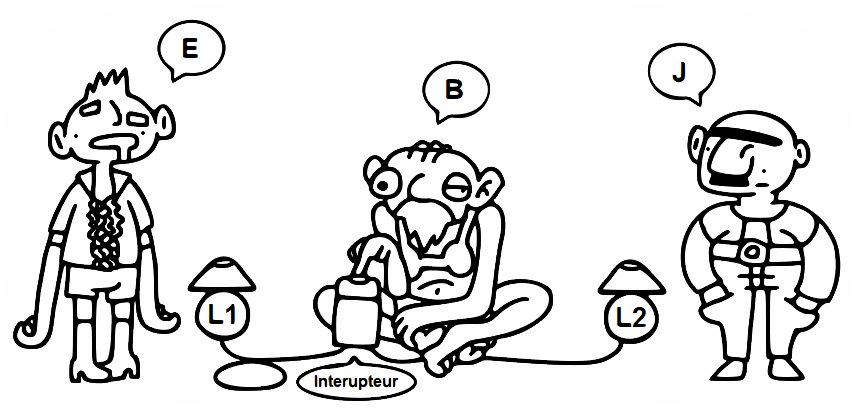
\includegraphics[scale=0.4]{../cours/la_science_pour_les_basios_by_eurydrama.png}
			\caption{Dispositif expérimental mettant en évidence le caractère relatif de la simultanéité.}
			\label{pluthaar}
		\end{figure}

		Pour être plus clairs, imaginons un exemple simple. Soit trois observateurs $B=$Bernard, $J=$Jean-Jacques, $E=$Eudes-Kévin, situés selon la figure \ref{pluthaar}. Les deux lampes $L_1$ et $L_2$ sont disposées à égales distances de Bernard. À $t=0$, Bernard appuie sur un interrupteur. Le signal électrique se propage le long des deux fils, et les deux lampes s'allument. Le signal lumineux met $\Delta t_1=L_1B/c=L_2B/c$ à parvenir à Bernard, celui-ci voit donc les deux lampes s'allumer en même temps. Cependant, pour Jean-Jacques, les choses sont différentes. En effet, comme $L_1J>L_2J$, ce gars-là verra la lampe $L_2$ s'allumer avant la lampe $L_1$. La situation est inverse pour Eudes-Kévin. Ainsi, la simultanéité pour un observateur n'implique pas la simultanéité pour tous les observateurs en théorie relativiste. Notons à ce stade que le principe de causalité n'est pas remis en question. En effet, l'allumage de la lampe $L_1$ n'est pas la cause de l'allumage de la lampe $L_2$, et réciproquement ; ces événements peuvent donc apparaître dans un ordre quelconque selon le référentiel. En revanche, que ce soit pour Jean-Jacques ou Eudes-Kévin, les deux verront Bernard appuyer sur l'interrupteur toujours avant l'allumage de l'une ou de l'autre lampe, à deux conditions : la vitesse de propagation du courant électrique est plus faible que la vitesse de la lumière, et les deux observateurs (Jean-Jacques et Eudes-Kévin) se déplacent eux-mêmes plus lentement que la lumière\footnote{Dans le cas où l'un des trois phénomènes est aussi rapide que la vitesse de la lumière, il peut au mieux y avoir simultanéité apparente.}. Malgré le caractère relatif du temps, mettons définitivement fin aux faux espoirs : la causalité est absolue dans la théorie relativiste de l'espace-temps. Cela sera aussi vrai en relativité générale. Il est absolument impossible de modifier son passé en théorie relativiste. Enfin, notons que la causalité absolue est une conséquence du caractère fini du maximum de la vitesse des propagations.

		Une autre conséquence du principe de relativité est que les solides indéformables n'existent pas. En effet, si c'était le cas, le choc d'un autre solide sur un solide donné impliquerait un mouvement d'ensemble comme conséquence d'un choc en un point de contact. Ainsi, un autre point du solide indéformable, éloigné du point de contact, serait animé d'un mouvement instantanément après le choc, ce qui est contraire avec la vitesse de propagation finie des informations. Les points du solide éloignés du point de contact doivent "attendre" que l'information de la perturbation du point de contact arrive jusqu'à eux, et cette information ne peut se transmettre instantanément.

		Énonçons une bonne fois pour toute le principe de relativité d'Einstein :

		\hspace{-0.5cm}\fbox{\parbox{\textwidth}{Les lois de la nature sont les mêmes dans tous les référentiels inertiels. De plus, la propagation des signaux et des interactions entre les corps admet une vitesse maximale universelle qui est la même dans tous les référentiels inertiels.}}

		Discutons un peu des conséquences de ce principe. Une autre façon de l'énoncer est de dire que le mouvement\footnote{Sous-entendu rectiligne uniforme.} est comme rien.  Toutes les expériences physiques donneront strictement les mêmes résultats dans tous les référentiels galiléens. Si vous changez d'un référentiel à un autre, la vitesse de la lumière sera toujours "infiniment" éloignée de vous. En effet, si vous accélérez pour gagner, mettons, $100\mathrm{km}/\mathrm{s}$, vous ne faites que passer d'un référentiel inertiel à un autre. Une fois que vous vous situez dans ce second référentiel inertiel, vous pouvez alors tout remettre à zéro et annuler votre vitesse. Du point de vue d'un observateur, la lumière est donc perpétuellement inateignable, quels que soient les efforts fournis. Un deuxième observateur qui voit le premier accélérer perpétuellement, ne le verra jamais dépasser la vitesse de la lumière ; il peut au mieux l'observer s'en approcher asymptotiquement, comme nous le montrerons bientôt. Le principe de relativité est une démocratisation des référentiels inertiels : ceux-ci se valent tous.

		Il suit aussi que la constante $c$ est une constante universelle de la physique. La vitesse de la lumière n'est pas le résultat de calculs, elle est profondément ancrée dans les postulats même de la théorie. Nous verrons également abondamment que les seuls protocoles expérimentaux fiables se fondent sur la propagation de la lumière. Les seules mesures fondamentales de distances sont en fait des mesures de temps de propagation de la lumière, que nous multiplions par $c$ pour obtenir des distances.

		Pour finir ce paragraphe d'introduction, discutons de la notion de théorie du champ. Deux objets ne peuvent interagir que via un champ d'interaction dont les modifications ne peuvent se propager que localement de proche en proche, et la vitesse de cette propagation est universellement (dans tous les référentiels inertiels) par la vitesse de la lumière. Comme nous le verrons, le champ lui-même est un objet physique. Conceptuellement, il faut donc comprendre que deux objets qui interagissent constituent en réalité trois objets physiques : les deux objets dont on souhaite déterminer théoriquement la dynamique, et le champ d'interaction entre ces deux objets. En théorie du champ, lorsqu'on place deux objets ensemble, on ne peut les étudier correctement qu'en étudiant trois objets.





	%\pagebreak


\part{Applications physiques, développements}


	\chapter{Problème à $N$ corps en relativité générale}

	\section{Introduction}

		Le problème à $N$ corps gravitationnel consiste à prédire le mouvement de $N$ corps en interaction gravitationnelle connaissant leurs positions et vitesses à un instant donné. Dans ce chapitre, nous allons montrer comment traîter ce problème avec le cadre de la théorie de la relativité générale. Contrairement à la théorie newtonienne, la première étape du problème à $N$ corps qui consiste à obtenir les équations du mouvement est beaucoup moins aisée. C'est surtout à cela que sera consacré ce chapitre. Une fois les équations du mouvement obtenues, leur résolution est un problème purement mathématique (ou numérique). L'objet de cet ouvrage se concentrant plus sur la théorie de la relativité générale, nous n'exposerons pas les méthodes de résolutions des équations du mouvement dans le détail. La dernière section de ce chapitre résumera les dernières avancées en terme de résolution, en accentuant l'aspect relativiste de la chose. Des références seront données pour qui compte approfondir ce problème.


	\section{Description géométrique relativiste du problème à $N$ corps}

		\subsection{Introduction et notations}
			Avant tout calcul prédictif il faut préciser le cadre géométrique dans lequel nous travaillons. En effet, les hypothèses physiques ont des manifestations géométriques, ce qui est très naturel dans une théorie comme la relativité générale. 

			Les lettres grecques minuscules $\alpha,\beta,\ldots$ désignes les 4 coordonnées $0,1,2,3$ de l'espace temps alors que les lettres latines minuscules $a,b,\ldots$ renvoient aux coordonnées spatiales $1,2,3$. Les convention de sommation d'Einstein sont bien évidemment adoptées sur les lettres grecques, mais aussi sur les lettres latines : ainsi,
			\begin{equation}
				A_iB^i \equiv A_1B^1 + A_2B^2+A_3B^3
			\end{equation}
			mais nous posons également
			\begin{equation}
				A^iB^i \equiv \delta_{ij}A^iB^j=A^1B^1+A^2B^2+A^3B^3.
			\end{equation}
			Nous serons amenés à faire des développements limités en $1/c$. C'est pourquoi nous adoptons les notations compactes suivantes. Pour tout champ scalaire $\Phi$,
			\begin{equation}
				\Phi = O(c^{-n}) \quad \Leftrightarrow \quad \Phi=O(n).
			\end{equation}
			Pour tout 4-vecteur de coordonnées $A^\mu$,
			\begin{equation}
				A^0=O(p)\quad\text{et}\quad A^i=O(q) \quad \Leftrightarrow \quad A^\mu=O(p,q). 
			\end{equation}
			Pour tout tenseur de rang 2 et de coordonnées $T^{\mu\nu}$,
			\begin{equation}
				T^{00}=O(p), \quad T^{0i}=O(q), \quad T^{i0}=O(q)\quad T^{ij}=O(r) \quad \Leftrightarrow \quad T^{\mu\nu}=O(p,q,r).
			\end{equation}
			Enfin, nous utilisons la convention des parenthèses pour symétriser un tenseur et des crochets pour l'antisymétriser :
			\begin{equation}\label{parent_sym}
				T^{(\mu\nu)}\equiv\frac{1}{2}(T^{\mu\nu}+T^{\nu\mu})
			\end{equation}
			\begin{equation}
				T^{[\mu\nu]}\equiv\frac{1}{2}(T^{\mu\nu}-T^{\nu\mu})
			\end{equation}

		\subsection{Choix du système de coordonnées}
			Dans le cadre d'une théorie relativiste, nous faisons l'hypothèse (forte) que les corps évoluent dans une variété $\mathscr{V}$  différentiable de dimension 4 parcourue par $N$ lignes d'univers $\mathscr{L}_A,\, A\in\{1,\ldots,N\}$. Soit $\mathscr{T}_A\subset \mathscr{V}$ un voisinage ouvert de $\mathscr{L}_A$. Soit $X^\mu_A$ un système de coordonnées décrivant $\mathscr{T}_A$ adapté à $\mathscr{L}_A$, c'est-à-dire qu'un paramétrage possible de $\mathscr{L}_A$ dans $\mathscr{T}_A$ est $X^\mu(P(s)\in\mathscr{L}_A)=(s,0,0,0),\, s\in\mathbb{R}$. La base naturelle associée à ce système de coordonnées le long de $\mathscr{L}_A$ est définie de la façon suivante :
			\begin{equation}
				e^A_\mu}(s) = \left.\frac{\partial}{\partial X_A^\mu}\right|_{P(s)\in\mathscr{L}_A}.
			\end{equation}
			Nous ajoutons aux $N$ systèmes de coordonnées adaptés aux $N$ lignes d'univers le système de coordonnées suivant. Nous supposons qu'il existe un système de coordonnées global décrivant tout $\mathscr{V}$ (donc incluant tous les $\mathscr{T}_A$) que nous noterons $x^\mu$. L'objet de toute cette section sera de décrire le changement de coordonnées de $X_A^\mu$ à $x^\mu$. À présent, considérons les $N$ changements de coordonnées :
			\begin{equation}
				x^\mu = f^\mu_A(X^\nu_A).
			\end{equation}
			Nous allons paramétriser ce changement de coordonnées en posant les définitions suivantes :
			\begin{equation}
				z^\mu_A (s) \equiv f^\mu(s,0,0,0)
			\end{equation}
			\begin{equation} \label{def_e_diff}
				e^\mu_{A,\nu}(s)\equiv \left.\frac{\partial f^\mu_A}{\partial X^\nu_A}\right|_{X^\mu=(s,0,0,0)}=\left.\frac{\partial f^\mu_A}{\partial X^\nu_A}\right|_{P(s)\in\mathscr{L}_A}
			\end{equation}
			\begin{equation}
				\xi^\mu_A(X^\nu_A)\equiv f^\mu_A(X^\nu_A)-f^\mu_A(s,0,0,0)-e^\mu_{A,j}X_A^j
			\end{equation}

			$z^\mu_A(s)$ n'est donc rien d'autre que la représentation paramétrique, dans le système de coordonnées $x^\mu$, de la ligne d'univers $\mathscr{L}_A$ paramétrisée par $s$.

			De ce fait, nous remarquons que
			\begin{equation}
				e^A_\mu}(s) = \left.\frac{\partial}{\partial X_A^\mu}\right|_{\mathscr{L}_A}=e^\nu_{A,\mu}e^A_\nu}(s) = \left.e^\nu_{A,\mu}\frac{\partial}{\partial x^\nu}\right|_{\mathscr{L}_A}.
			\end{equation}
			Remarquons également que
			\begin{equation}
				e^\mu_{A,0}=\frac{\d z^\mu_A}{\d s}.
			\end{equation}
			Avec ces notations, le changement de coordonnées s'écrit de la façon suivante :
			\begin{equation}
				x^\mu(X^\nu}) = z^\mu(X^0)+e^\mu_{\phantom{x}i}X^i + \xi^\mu(X^\nu})
			\end{equation}
			où nous avons sous-entendu l'indice $A$ pour éviter d'alourdir les notations. Comme nous supposons que toutes les fonctions considérées sont différentiables\footnote{Probablement l'hypothèse la plus lourde de toute la théorie de la relativité générale...}, cette dernière relation combinée avec la partie spatiale de définition \ref{def_e_diff} nous prouvent que
			\begin{equation}
				\xi^\mu(X^\nu}) = O((X^i)^2)
			\end{equation}
			quand $X^i\rightarrow 0$ pour $X^0$ fixé.
			La matrice jacobienne de ce changement de variables, dont nous définissons les coordonnées ainsi :
			\begin{equation}
				A^\mu_{\phantom{x}\nu}\equiv\frac{\partial x^\mu}{\partial x^\nu}
			\end{equation}
			s'écrit
			\begin{equation}
				A^\mu_{\phantom{x}0}=e^\mu_{\phantom{x}0}(s) + \frac{\d e^\mu_{\ i}(s)}{\d s} X^i + \frac{\partial \xi ^\mu}{\partial s}
			\end{equation}
			\begin{equation}
				A^\mu_{ \ k}=e^\mu_{\phantom{x}k}(s)+\frac{\partial \xi^\mu}{\partial X^k}
			\end{equation}
			Remarquons que jusqu'ici toutes les définitions se passent du tenseur métrique et sont purement topologiques. À présent il est temps d'introduire les hypothèses physiques du modèle et leur manifestations dans la courbure de l'espace-temps.

		\subsection{Hypothèses physiques du modèle}
			Nous supposons que les corps sont lents devant la vitesse de la lumière, et aussi qu'ils génèrent de faibles champs gravitationnels, c'est-à-dire modifiant peu le tenseur métrique par rapport au tenseur métrique de Minkowski dont nous notons les coordonnées $\eta_{\mu\nu}$.
			L'hypothèse du mouvement lent s'écrit
			\begin{equation}
				\frac{\d z^i}{\d s} = \frac{\d z^i}{c \, \d \tau} = O(1)
			\end{equation}
			L'hypothèse du champ faible combinée avec l'hypothèse du mouvement lent nous amène à supposer qu'il existe $N+1$ systèmes de coordonnées $x^\mu$ et $X^\mu_A,\ A\in\{1,\ldots,N\}$ tels qu'en chacun de ces systèmes de coordonnées, le tenseur métrique vérifie :
			\begin{equation}\label{hyp_g}
				g_{\mu\nu}(x^\alpha)-\eta_{\mu\nu}=h_{\mu\nu}(x^\alpha)=O(2,3,2),
			\end{equation}
			\begin{equation}\label{hyp_G}
				G^A_{\mu\nu}(X^\alpha_A)-\eta_{\mu\nu}=H^A_{\mu\nu}=O(2,3,2).
			\end{equation}
			L'hypothèse du mouvement lent s'écrit ainsi :
			\begin{equation}
				A^\mu_{\ \nu}=O(0,1,0). \label{hyp_v}
			\end{equation}
			Ces hypoythèses peuvent d'emblée mener à quelques résultats intéressants. La loi de transformation des composantes du tenseur métrique s'écrit
			\begin{equation}
				G_{\alpha\beta}=A^\mu_{\ \alpha}A^\nu_{\ \beta}g_{\mu\nu}
			\end{equation}
			Les hypothèses \ref{hyp_g} et \ref{hyp_G} conduisent immédiatement à 
			\begin{equation}\label{pn_contrainte}
				\eta_{\mu\nu}A^\mu_{\ \alpha}A^\nu_{\ \beta} = \eta_{\alpha\beta}+O(2,3,2).
			\end{equation}
			Le tenseur métrique ayant disparu, cette relation ne donne que des contraintes mathématiques sur la structure du changement de coordonnées $x^\mu=f^\mu(X^\nu)$. La relation \ref{pn_contrainte} étant vraie pour tous $X^i$, nous pouvons effectuer un développement limité et obtenir des égalités correspondantes aux ordres $O((X^i)^0)$, $O((X^i)^1)$ et $O((X^i)^2)$. Pour simplifier les notations, nous notons $O((X^i)^n)\equiv O(X^n)$. Comme nous avons 
			\begin{equation}
				A^\mu_{\ \nu}=e^\mu_{\ \nu}+O(X) 	
			\end{equation}
			l'ordre $O(X^0)$ de l'équation \ref{pn_contrainte} implique que
			\begin{equation}\label{o_z_pn_a}
				\eta_{\mu\nu}e^\mu_{\ \alpha}e^\nu_{\ \beta}=\eta_{\alpha\beta}+O(2,3,2).
			\end{equation}

			La composante $(\alpha,\beta)=(0,0)$ de \ref{o_z_pn_a} donne 
			\begin{equation}
				-e^0_{\ 0}^2 + e^i_{\ 0}e^i_{\ 0} = -1 + O(2)	
			\end{equation}
			mais comme $e^i_{\ 0}=\d z^i / \d s = O(1)$, nous pouvons oublier le deuxième terme du membre de gauche et obtenir $e^0_{\ 0}^2=1+O(2)$ ce qui équivaut à 
			\begin{equation}\label{e_0_0}
				e^0_{\ 0}=1+O(2)	
			\end{equation}

			La composante $0a$ de la relation \ref{o_z_pn_a} nous donne
			\begin{equation}
				-e^0_{\ a}e^0_{\ 0}+e^i_{\ a}e^i_{\ 0}=O(3)
			\end{equation}
			Mais comme $e^0_{\ a}=O(1)$, nous avons, en vertu de \ref{e_0_0},
			\begin{equation}
				e^0_{\ a}e^0_{\ 0}=e^0_{\ a}+O(3)
			\end{equation}
			et donc
			\begin{equation}
				e^0_{\ a}=e^i_{\ a}e^i_{\ 0}+O(3)=e^i_{\ a}\frac{\d z^i}{\d s} + O(3).
			\end{equation}
			La composante $ab$ de \ref{o_z_pn_a} donne, grâce à $e^0_{\ a}e^0_{\ b}=O(2)$ :
			\begin{equation}
				e^i_{\ a}e^i_{\ b}=\delta_{ab}+O(2). \label{rotation_ab}
			\end{equation}
			Ensuite, la composante $00$ de l'équation  \ref{pn_contrainte} s'écrit
			\begin{equation}\label{dev_pn_contrainte}
				-\left(e^0_{\ 0}+ \frac{\d e^i_{\ a}}{\d s} X^a \right)^2 + \left( e^i_{\ 0} + \frac{\d e^i_{\ a}}{\d s} X^a \right)\left( e^i_{\ 0} + \frac{\d e^i_{\ a}}{\d s} X^a \right)=-1+O(2).
			\end{equation}
			Tenant compte de ceci et ne gardant que l'ordre $O(X)$ de l'équation \ref{dev_pn_contrainte}, nous obtenons :
			\begin{equation}
				-e^0_{\ 0}\frac{\d e^i_{\ a}X^a}{\d s} + 2 e^i_{\ 0}\frac{\d e^i_{\ a}}{\d s}X^a=O(2)
			\end{equation}
			Par ailleurs, nous avons
			\begin{equation}
				\frac{\d}{\d s}=\frac{\d}{c\, \d \tau}=O(1).
			\end{equation}
			et $e^i_{\ 0}=O(1)$ donc $e^i_{\ 0}\d e^i_{\ a}/\d s=O(2)$ ; de plus, $e^0_{\ 0}=1+O(2)$ ; nous en déduisons :
			\begin{equation}
				\frac{\d e^i_{\ a}}{\d s}=O(2).
			\end{equation}
			La composante $ab$ de l'équation \ref{dev_pn_contrainte} s'écrit :
			\begin{equation}
				-\left(e^0_{\ a}+\frac{\partial \xi^0}{\partial X^a}\right)\left(e^0_{\ b}+\frac{\partial \xi^0}{\partial X^b}\right)
				+\left( e^i_{\ a} + \frac{\partial \xi^i}{\partial X^a} \right)\left( e^i_{\ b} + \frac{\partial \xi^i}{\partial X^b} \right)
				=\delta_{ab}+O(2).
			\end{equation}
			L'ordre $O(X))$ de cette équation s'écrit :
			\begin{equation}\label{o_1_pn_ab}
				-2e^0_{\ (a}\frac{\partial \xi^0}{\partial X^{b)}}+2e^i_{\ (a}\frac{\partial \xi^i}{\partial X^{b)}}=O(2)
			\end{equation}
			où la notation de symétrisation \ref{parent_sym} a été utilisée.
			Mais comme $A^0_{\ i}=O(1)$, cela est vrai à l'ordre $O(X^0)$ et l'ordre $O(X)$, donc $e^0_{\ i}=O(1)$ et $\partial \xi^0/\partial X^i=O(1)$, et ainsi le premier terme de \ref{o_1_pn_ab} est de l'ordre $O(2)$ et peut être négligé. D'après \ref{rotation_ab}, $e^i_{\ j}=O(0)$. Nous en déduisons que $\partial \xi^i/\partial X^a=O(2)$, et comme la dérivation selon $X^a$ ne change pas l'ordre en $1/c$ et que $\xi^\mu$ est quadratique en $X^a$, nous en déduisons que $\xi^\i=O(2)$.
			La composante $a0$ de l'équation \ref{dev_pn_contrainte} s'écrit :
			\begin{equation}
				-\left(e^0_{\ a}+\frac{\partial \xi^0}{\partial X^a}\right)\left( e^0_{\ 0}+\frac{\d e^0_{\ j}}{\d s}X^j +\frac{\partial \xi^0}{\partial s} \right)
				+\left( e^i_{\ a} + \frac{\partial \xi^i}{\partial X^a} \right)\left( e^i_{\ 0} + \frac{\d e^i_{\ j}}{\d s}X^j +\frac{\partial \xi^i}{\partial s} \right) 
				= O(3).
			\end{equation}
			Cette fois, nous ne gardons que l'ordre $O(X^2)$ de cette équation pour finalement obtenir :
			\begin{equation}
				-\frac{\partial \xi^0}{\partial X^a}\frac{\d e^0_{\ j}}{\d s}X^j-e^0_{\ a}\frac{\partial \xi^0}{\partial s} + e^i_{\ a}\frac{\partial \xi^i}{\partial s} + \frac{\partial \xi^i}{\partial s}\frac{\d e^i_{\ j}}{\d s}X^j = O(3)
			\end{equation}
			Mais un instant d'analyse montre que le premier terme est de l'ordre $O(3)$ ($\d e^0_{\ a}/\d s=O(2)$ et $\partial \xi^0/\partial X^i=O(1)$), ainsi que le troisième ($\partial \xi^i/\partial s=O(3)$) alors que le dernier terme est de l'ordre $O(4)$ (\partial $\xi^i/\partial s=O(2)$ et $\d e^i_{\ a}/\d s=O(2)$). Ainsi, il ne reste que
			\begin{equation}
				e^0_{\ a}\frac{\partial \xi^0}{\partial s}=O(3)
			\end{equation}
			ce qui prouve que $\partial \xi^0/\partial s=O(2)$ et donc que $\xi^0=O(3)$. 

			Résumons les résultats de tout ce paragraphe. Le changement de coordonnées pour passer du repérage local au repérage global est paramétrisé de la façon suivante, ordre par ordre en $O(X)$ :
			\begin{equation}
				x^\mu(X^\nu)=z^\mu(s)+e^\mu_{\ i}(s)X^i + \xi^\mu(X^\nu).
			\end{equation}
			Avec $s\equiv X^0$.
			Dans cette paramétrisation, les approximation post-newtoniennes \ref{hyp_g}, \ref{hyp_G} et \ref{hyp_v} sont mathématiquement équivalentes à la suite d'égalités suivantes :
			\begin{eqnarray}
				e^0_{\ 0}(s)&\equiv&\frac{\d z^0}{\d s}=1+O(2) \\
				e^0_{\ a}(s)&=&e^i_{\ a}(s)\frac{\d z^i}{\d s}+O(3) \\
				e^i_{\ 0}&\equiv&\frac{\d z^i}{\d s} \\
				e^i_{\ a}(s)e^i_{\ b}(s)&=&\delta_{ab}+O(2) \\
				\frac{\d e^i_{\ a}}{\d s}&=&O(2) \\
				\xi^0&=&O(3) \\
				\xi^i&=&O(2).
			\end{eqnarray}

		\subsection{Coordonnées spatiales cartésiennes, contraintes sur les paramètres $z-e-\xi$}

			Pour donner des contraintes géométriques supplémentaires, nous allons devoir anticiper un tout petit peu et considérer les équations d'Einstein.


	\section{Action du problème à $N$ corps}

		Nous souhaitons obtenir les équations du mouvement à partir d'un principe variationnel. Pour cela nous devons décrire l'action du champ gravitationnel ainsi que l'action de la matière des corps en mouvement. L'action du champ gravitationnel a déjà été discutée au chapitre \ref{action_champ} de la partie 1 :
		\begin{equation}
			S_g = \int R \sqrt{-g} \, \d^4 \bm{x}
		\end{equation}

		\subsection{Densité invariante, masses des corps}

			Soit un champ de matière quelconque décrit par une densité de masse locale au repos $\rho$. Considérons un référentiel comobile avec la matière en un point $\bm{r}$ donné de l'espace. Dans ce référentiel, entre $t$ et $t+dt$ la masse totale contenue dans un élément de volume ne doit pas varier :
			\begin{equation}
				\frac{\d(\rho \, d^3\bm{x})}{\d t} = 0
			\end{equation}
			En faisant un bilan sur l'élément de volume $\d^3\bm{v}$ il est aisé de montrer que dans le référentiel comobile cette équation est équivalente à l'équation de continuité :
			\begin{equation}
				\rho_{,t} + (\rho v^i)_{,i} = 0		
			\end{equation}	
			Lors d'un changement local de référentiel via une transformation de Lorentz, cette équation devient simplement :
			\begin{equation}
				(\rho u^\mu)_{,\mu}=0
			\end{equation}
			Pour passer en espace courbe il suffit d'écrire :
			\begin{equation}
				(\rho u^\mu)_{;\mu}=0
			\end{equation}
			Or comme pour tout 4-vecteur $A^\mu$, nous avons 
			\begin{equation}
				(A^\mu)_{;\mu}=\frac{1}{\sqrt{-g}}(\sqrt{-g}A^\mu)_{,\mu}
			\end{equation}
			nous en déduisons, avec $u^i=u^0v^i$ :
			\begin{equation}
				(\rho\sqrt{-g}u^0)_{,0}+(\rho\sqrt{-g}u^0v^i)_{,i}=0
			\end{equation}
			de telle sorte que la densité conservée $\rho^*$ définie par
			\begin{equation}
				\rho^*\equiv \rho \sqrt{-g}u^0
			\end{equation}
			vérifie l'équation de continuité
			\begin{equation}
				\rho^*_{,t}+(\rho^*v^i)_{,i}=0
			\end{equation}
			pour un système de coordonnées $(t,\bm{x})$ quelconque.

			On en déduit que pour toute fonction $f(\bm{x},t)$ s'annulant au delà du volume $V$, nous avons :
			\begin{equation}
				\frac{\d}{\d t} \int_V \rho^* f(\bm{x},t) \, \d^3\bm{x} = \int_V \rho^* \frac{\d f}{\d t} \,\d^3\bm{x} 
			\end{equation}

			En posant $f\equiv 1$ nous pouvons définir la masse invariante d'un corps $A$ :
			\begin{equation}
				M_A = \int_A \rho^* \d^3\bm{x} = \int_A \rho \sqrt{-g} u^0 \, \d^3\bm{x}
			\end{equation}

			La masse invariante d'un système physique $\mathscr{S}$ s'exprime donc de la façon suivante :
			\begin{equation}
				M_{\mathscr{S}}=\int_{\mathscr{S}} \rho \sqrt{-g} u^0 \, \d^3\bm{x} 
			\end{equation}
			et son énergie au repos est simplement $M_\mathscr{S}c^2$. Du point de vue d'un observateur $\mathscr{O}$ de temps propre $s$ ayant choisi un système de coordonnées $t,\bm{x}$, il semble naturel d'intégrer cette énergie invariante le long de sa ligne d'univers entre deux dates pour définir l'action de la matière mesurée par $\mathscr{O}$. Nous posons donc :
			\begin{equation}
				S_m = \alpha \int \int c^2 \rho \sqrt{-g} u^0 \, \d^3\bm{x} \, \d s_\mathscr{O} = \int c^2 \rho \sqrt{-g} \, \d^4\bm{x} 
			\end{equation}
			où $\alpha$ est une constante multiplicative. Pour trouver $\alpha$, nous demandons que cette action très générale coïncide avec le cas particulier de l'action de $N$ corps ponctuels qui n'interagissent pas :
			\begin{equation}
				S_{N\phantom{l}corps}=\sum_A M_A c^2 \int \d s_A
			\end{equation}
			où $M_A$ est la masse invariante au repos du corps $A$

			Pour retrouver cette action, nous pouvons découper l'intégration volumique sur chaque corps et écrire :
			\begin{equation}
				S_{N\phantom{l}corps}= \alpha c^2 \sum_A \int \left( \int_A \rho \sqrt{-g} u^0 \, \d^3\bm{x} \right) \d x^0 = \sum_A \alpha c^2 \int \rho_A \sqrt{-g} u^0 \d^4\bm{x}
			\end{equation}
			Comme le corps $A$ est supposé ponctuel\footnote{Nous étudierons les corps non ponctuels très bientôt...}, $\rho$ est proportionnel à $\delta^3(\bm{x}-\bm{x}_A)$, de telle sorte qu'il est licite d'écrire :
			\begin{equation}
				M_A = \int_A \rho \sqrt{-g} u^0 \, \d^3\bm{x} = u^0_A \int_A \rho \sqrt{-g} \, \d^3\bm{x} 
			\end{equation}
			où $u^\mu_A$ est la quadrivitesse du point $A$. Ainsi, nous obtenons :
			\begin{equation}
				S_{N\phantom{l}corps}=sum_A \alpha c^2 \int M_A \frac{\d x^0}{u^0_A} = \sum_A \alpha c^2 M_A \int \d s_A
			\end{equation}
			qui coïncide avec l'expression de l'action de $N$ corps ponctuels non interagissant en posant $\alpha=1$.
			Ainsi l'action totale de la matière d'un système physique donné s'écrit :


	\section{Template}
		\begin{post}
			postulat
		\end{post}
		\begin{theorem}
			théorème
		\end{theorem}

		\begin{proof}
			preuve
			\end{proof}


		\begin{figure}
			\centering
			\includegraphics[scale=0.07]{figures/figure.jpg}
			\caption{Figure}
		\label{fig}
		\end{figure}


	\chapter{Titre}
	\section{Template}
		\begin{post}
			postulat
		\end{post}
		\begin{theorem}
			théorème
		\end{theorem}

		\begin{proof}
			preuve
		\end{proof}


		\begin{figure}
			\centering
			\includegraphics[scale=0.07]{figures/figure.jpg}
			\caption{Figure}
			\label{fig}
		\end{figure}


	\chapter{Titre}
        \section{Template}
                \begin{post}
                        postulat
                \end{post}
                \begin{theorem}
                        théorème
                \end{theorem}

                \begin{proof}
                        preuve
                \end{proof}


                \begin{figure}
                        \centering
                        \includegraphics[scale=0.07]{figures/figure.jpg}
                        \caption{Figure}
                        \label{fig}
                \end{figure}


	\chapter{Titre}
        \section{Template}
                \begin{post}
                        postulat
                \end{post}
                \begin{theorem}
                        théorème
                \end{theorem}

                \begin{proof}
                        preuve
                \end{proof}


                \begin{figure}
                        \centering
                        \includegraphics[scale=0.07]{figures/figure.jpg}
                        \caption{Figure}
                        \label{fig}
                \end{figure}









%%%%%%%%%%%%%%%%%%%%%%%%%%%%%
%Intro
%%%%%%%%%%%%%%%%%%%%%%%%%%%%%
%\chapter{Introduction}
\chapter*{Conclusion} \addcontentsline{toc}{chapter}{Conclusion}  %Tout ce bazar permet d'avoir l'intro dans la table des matières sans la numéroter
\markboth{Conclusion}{Conclusion}













%%%%%%%%%%%%%%%%%%%%%%%%%%%%%%
%Bibliographie
%%%%%%%%%%%%%%%%%%%%%%%%%%%%%
%\bibliographystyle{plain}
\bibliographystyle{plain}
\bibliography{../bibfile/bibfile.bib}



%%%%%%%%%%%%%%%%%%%%%%%%%%%%
%Annexe
%%%%%%%%%%%%%%%%%%%%%%%%%%%
%décommenter la ligne suivante si besoin :
%\appendix





\end{document}

